\chapter{Preambolo}
\section{Rango di una matrice}
Consideriamo una matrice $A \in \mathbb{R} ^ {m \times n}$
\begin{definition}{Rango di una Matrice}
    Il rango di una matrice indica il numero di righe (o colonne, dipende da che notazione usiamo), lineramente indipendenti.
\end{definition}
\begin{proposition}{Rango Massimo di una Matrice}
Data una matrice \(A \in \mathbb{R}^{m \times n}\), il suo rango massimo è
\[
\boxed{\operatorname{rank}(A) \leq \min(m,n)}
\]
\end{proposition}
Perchè intuitivamente si ha questa proprietà?
Immagina avere una matrice dove i vettori sono sulle righe:
\[
A=
\begin{pmatrix}
1&0\\
0&1\\
1&1
\end{pmatrix}
\]
In questa matrice il rango massimo è 2, questo perchè in $\mathbb{R}^2$, al massimo due vettori possono essere lineramente indipendenti, se ne aggiungo un terzo, questo sarà sicuramamente combinazione lineare degli altri due. \\
Consideriamo questa altra matrice:
\[
A=
\begin{pmatrix}
1&0&1\\
0&1&0
\end{pmatrix}
\]
In questa matrice il rango massimo è sempre 2, questo perchè ci sono due vettori sulle righe.


\subsection{Cosa succede quando il rango è massimo ?}

Sia $R \in \mathbb{R}^{N \times M}$ una matrice con $N$ righe e $M$ colonne.

Il \textbf{rango} di una matrice è definito come il massimo numero di righe (o, equivalentemente, di colonne) linearmente indipendenti.

Per qualsiasi matrice vale la seguente proprietà:

\[
    \operatorname{rank}(R) \leq \min\{N,M\}.
\]

Il rango non può quindi superare il numero di righe né il numero di colonne della matrice.

Si dice che una matrice ha \textbf{rango massimo} (o \textit{full rank}) quando:

\[
    \boxed{\operatorname{rank}(R) = \min\{N,M\}.}
\]

In questo caso, la matrice contiene il massimo numero possibile di vettori linearmente indipendenti.

\paragraph{Caso 1: $N < M$ (più colonne che righe)}

Se la matrice ha più colonne che righe, il rango massimo è:

\[
    \operatorname{rank}(R) = N.
\]

Questo implica che:
\begin{itemize}
    \item Le $N$ righe sono tutte linearmente indipendenti.
    \item Esistono $N$ colonne linearmente indipendenti.
    \item Le $M$ colonne non possono essere tutte linearmente indipendenti, poiché $M > N$ e ciascuna colonna appartiene a $\mathbb{R}^N$.
\end{itemize}

Ad esempio, per una matrice $R \in \mathbb{R}^{3 \times 5}$, il rango massimo è $3$. Le tre righe possono essere tutte linearmente indipendenti, mentre tra le cinque colonne al massimo tre possono esserlo.

\paragraph{Caso 2: $N > M$ (più righe che colonne)}

Se la matrice ha più righe che colonne, il rango massimo è:

\[
    \operatorname{rank}(R) = M.
\]

Questo implica che:
\begin{itemize}
    \item Le $M$ colonne sono tutte linearmente indipendenti.
    \item Esistono $M$ righe linearmente indipendenti.
    \item Le $N$ righe non possono essere tutte linearmente indipendenti, poiché $N > M$ e ciascuna riga appartiene a $\mathbb{R}^M$.
\end{itemize}

\paragraph{Caso 3: $N = M$ (matrice quadrata)}

Se la matrice è quadrata, il rango massimo è:

\[
    \operatorname{rank}(R) = N = M.
\]

In questo caso:
\begin{itemize}
    \item Tutte le righe sono linearmente indipendenti.
    \item Tutte le colonne sono linearmente indipendenti.
    \item La matrice è invertibile, ossia esiste $R^{-1}$.
    \item Il determinante è diverso da zero: $\det(R) \neq 0$.
\end{itemize}

\paragraph{Interpretazione geometrica}

Le colonne di una matrice $R \in \mathbb{R}^{N \times M}$ sono vettori appartenenti allo spazio $\mathbb{R}^{N}$, mentre le righe sono vettori appartenenti a $\mathbb{R}^{M}$.

In uno spazio vettoriale di dimensione $d$, non possono esistere più di $d$ vettori linearmente indipendenti.

Pertanto, se $M > N$, le $M$ colonne di $R$ non potranno mai essere tutte linearmente indipendenti, indipendentemente dai valori contenuti nella matrice.

\paragraph{Osservazione fondamentale}

Avere rango massimo \textbf{non significa necessariamente che tutte le righe e tutte le colonne siano linearmente indipendenti}.

Significa, invece, che la matrice possiede il massimo numero di vettori linearmente indipendenti consentito dalle sue dimensioni:

\[
    \boxed{\operatorname{rank}(R) = \min\{N,M\}.}
\]

Solo nel caso di una matrice quadrata a rango massimo si può affermare che tutte le righe e tutte le colonne sono contemporaneamente linearmente indipendenti.


 \section{Linearmente Indipendenza}

Due o più vettori si dicono **linearmente indipendenti** quando nessuno di essi può essere espresso come combinazione lineare degli altri. Nel caso particolare di due vettori, questo significa che uno non può essere ottenuto moltiplicando l'altro per uno scalare.

Al contrario, due o più vettori si dicono **linearmente dipendenti** quando almeno uno di essi può essere espresso come combinazione lineare degli altri.

\subsection{Interpretazione geometrica nel piano}

Consideriamo due vettori appartenenti allo spazio \(\mathbb{R}^2\). Possiamo interpretarli geometricamente come frecce che partono dall'origine del piano cartesiano e terminano nei punti individuati dalle loro coordinate.

\subsubsection{Vettori linearmente indipendenti}

Consideriamo i seguenti vettori:

\[
v_1 =
\begin{pmatrix}
1\\
0
\end{pmatrix},
\qquad
v_2 =
\begin{pmatrix}
0\\
1
\end{pmatrix}.
\]

Il vettore \(v_1\) è diretto orizzontalmente verso destra, mentre il vettore \(v_2\) è diretto verticalmente verso l'alto. I due vettori hanno quindi direzioni differenti e non appartengono alla stessa retta passante per l'origine.

Per verificare che siano linearmente indipendenti, consideriamo l'equazione:

\[
\alpha v_1+\beta v_2=
\begin{pmatrix}
0\\
0
\end{pmatrix}.
\]

Sostituendo i vettori otteniamo:

\[
\alpha
\begin{pmatrix}
1\\
0
\end{pmatrix}
+
\beta
\begin{pmatrix}
0\\
1
\end{pmatrix}
=
\begin{pmatrix}
0\\
0
\end{pmatrix}.
\]

Da cui segue:

\[
\begin{cases}
\alpha=0\\
\beta=0
\end{cases}
\]

L'unica combinazione lineare che restituisce il vettore nullo è quindi quella in cui entrambi i coefficienti sono nulli. I due vettori sono pertanto linearmente indipendenti.

\paragraph{Significato geometrico.}

Due vettori linearmente indipendenti in \(\mathbb{R}^2\) individuano due direzioni distinte. Combinandoli linearmente, possiamo ottenere qualsiasi vettore del piano:

\[
\alpha v_1+\beta v_2
=
\begin{pmatrix}
\alpha\\
\beta
\end{pmatrix}.
\]

Infatti, scegliendo opportunamente i coefficienti \(\alpha\) e \(\beta\), possiamo raggiungere qualsiasi punto del piano cartesiano.

\subsubsection{Vettori linearmente dipendenti}

Consideriamo ora i vettori:

\[
v_1 =
\begin{pmatrix}
1\\
2
\end{pmatrix},
\qquad
v_2 =
\begin{pmatrix}
2\\
4
\end{pmatrix}.
\]

Osserviamo che il secondo vettore è il doppio del primo:

\[
v_2=2v_1.
\]

Pertanto, i due vettori hanno la stessa direzione e appartengono alla medesima retta passante per l'origine.

Per determinare l'equazione di questa retta, interpretiamo i vettori come punti del piano cartesiano.

Il primo vettore individua il punto \(P_1=(1,2)\), mentre il secondo individua il punto \(P_2=(2,4)\).

Entrambi i punti soddisfano la relazione:

\[
\boxed{y=2x}
\]

Infatti:
\begin{itemize}
    \item Per \(P_1=(1,2)\), abbiamo \(2=2\cdot 1\).
    \item Per \(P_2=(2,4)\), abbiamo \(4=2\cdot 2\).
\end{itemize}

La retta \(y=2x\) passa anche per l'origine \((0,0)\), poiché \(0=2\cdot 0\).

\paragraph{Verifica dell'indipendenza lineare.}

Per verificare che i vettori siano linearmente dipendenti, cerchiamo una combinazione lineare che restituisca il vettore nullo con coefficienti non entrambi nulli:

\[
\alpha v_1+\beta v_2=
\begin{pmatrix}
0\\
0
\end{pmatrix}.
\]

Sostituendo:

\[
\alpha
\begin{pmatrix}
1\\
2
\end{pmatrix}
+
\beta
\begin{pmatrix}
2\\
4
\end{pmatrix}
=
\begin{pmatrix}
0\\
0
\end{pmatrix}.
\]

Otteniamo il sistema:

\[
\begin{cases}
\alpha+2\beta=0\\
2\alpha+4\beta=0
\end{cases}
\]

Le due equazioni sono equivalenti. Esistono quindi infinite soluzioni non banali; ad esempio, scegliendo \(\alpha=-2\) e \(\beta=1\), si ottiene:

\[
-2v_1+v_2=
\begin{pmatrix}
0\\
0
\end{pmatrix}.
\]

I due vettori sono dunque linearmente dipendenti.

\paragraph{Significato geometrico.}

Combinando linearmente due vettori dipendenti, possiamo ottenere soltanto vettori appartenenti alla retta che li contiene. Non possiamo generare qualsiasi vettore del piano, perché i due vettori non introducono due direzioni distinte.

\subsection{Riepilogo geometrico}

Nel piano \(\mathbb{R}^2\), per due vettori non entrambi nulli, possiamo riassumere il concetto nel modo seguente:

\begin{itemize}
    \item \textbf{Vettori linearmente indipendenti:} i vettori non appartengono alla stessa retta passante per l'origine. Generano tutto il piano \(\mathbb{R}^2\).
    \item \textbf{Vettori linearmente dipendenti:} i vettori appartengono alla stessa retta passante per l'origine. Generano al massimo una retta.
\end{itemize}

\textbf{Attenzione:} se almeno uno dei vettori è il vettore nullo, i vettori sono linearmente dipendenti. Inoltre, nel caso di due vettori non nulli, essere sulla stessa retta passante per l'origine equivale a essere multipli scalari l'uno dell'altro.

\subsection{Collegamento con le matrici}

Il concetto di indipendenza lineare è utile anche nello studio delle matrici, in particolare nella Ricerca Operativa.

Consideriamo una matrice le cui colonne sono due vettori:

\[
A=
\begin{pmatrix}
1 & 2\\
2 & 4
\end{pmatrix}.
\]

Le colonne sono:

\[
A_1=
\begin{pmatrix}
1\\
2
\end{pmatrix},
\qquad
A_2=
\begin{pmatrix}
2\\
4
\end{pmatrix}.
\]

Poiché \(A_2=2A_1\), le colonne sono linearmente dipendenti e la matrice non ha rango massimo.

Al contrario, se le colonne sono linearmente indipendenti, descrivono direzioni distinte. In particolare, una matrice quadrata \(2\times 2\) ha rango massimo pari a \(2\) se e solo se le sue due colonne sono linearmente indipendenti.

Questo permette di collegare l'interpretazione geometrica dei vettori al concetto di rango di una matrice.



\section{Funzioni Convesse}

\subsection{Definizione Matematica}

Sia $I \subseteq \mathbb{R}$ un intervallo (limitato o illimitato). Una funzione $f: I \to \mathbb{R}$ si dice \textbf{convessa} su $I$ se, per ogni coppia di punti $x_1, x_2 \in I$ e per ogni $t \in [0, 1]$, si ha:
\begin{equation}
    f(t x_1 + (1-t) x_2) \le t f(x_1) + (1-t) f(x_2)
\end{equation}

Se la disuguaglianza vale in senso stretto per ogni $x_1 \neq x_2$ e per ogni $t \in (0, 1)$, ovvero:
\begin{equation}
    f(t x_1 + (1-t) x_2) < t f(x_1) + (1-t) f(x_2)
\end{equation}
la funzione si dice \textbf{strettamente convessa} su $I$.

\newpage

\paragraph{Interpretazione algebrica:} Il punto $x_t = t x_1 + (1-t) x_2$ rappresenta un generico punto compreso nell'intervallo $[x_1, x_2]$. La quantità $t f(x_1) + (1-t) f(x_2)$ rappresenta la quota corrispondente a $x_t$ sulla corda (segmento) che congiunge i punti $(x_1, f(x_1))$ e $(x_2, f(x_2))$.
Invece la quantità $f(t x_1 + (1-t) x_2)$, rappresenta la quota della funzione di un punto compreso nell'intervallo $[x_1, x_2]$.

Si deve avere che la quotà della funzione di un punto compreso nell'intervallo $[x_1, x_2]$, deve essere minore della quota corrispondente al segmento che congiunge $(x_1, f(x_1))$ e $(x_2, f(x_2))$.

\begin{figure}[htbp]
        \centering
        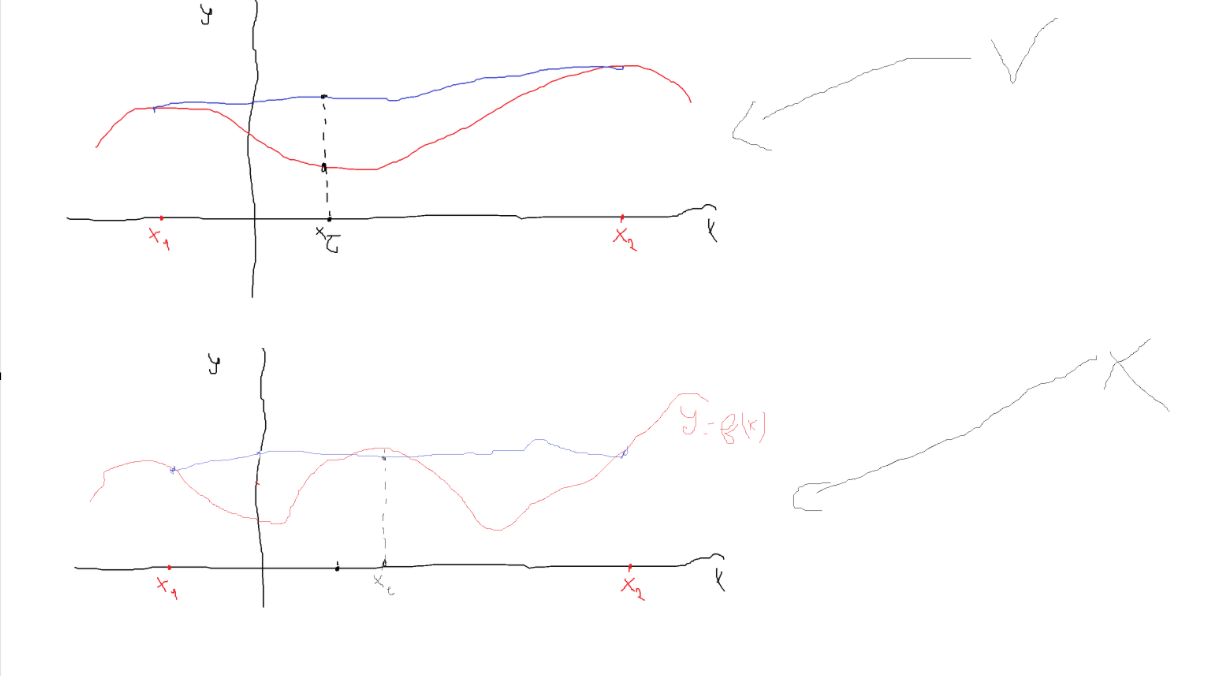
\includegraphics[width=0.8\textwidth]{_files/_images/28.png}
        \caption{Sopra vi è una funzione convessa, sotto no}
        \label{fig:mia_immagine}
\end{figure}